% Options for packages loaded elsewhere
\PassOptionsToPackage{unicode}{hyperref}
\PassOptionsToPackage{hyphens}{url}
%
\documentclass[
  ignorenonframetext,
]{beamer}
\usepackage{pgfpages}
\setbeamertemplate{caption}[numbered]
\setbeamertemplate{caption label separator}{: }
\setbeamercolor{caption name}{fg=normal text.fg}
\beamertemplatenavigationsymbolsempty
% Prevent slide breaks in the middle of a paragraph
\widowpenalties 1 10000
\raggedbottom
\setbeamertemplate{part page}{
  \centering
  \begin{beamercolorbox}[sep=16pt,center]{part title}
    \usebeamerfont{part title}\insertpart\par
  \end{beamercolorbox}
}
\setbeamertemplate{section page}{
  \centering
  \begin{beamercolorbox}[sep=12pt,center]{part title}
    \usebeamerfont{section title}\insertsection\par
  \end{beamercolorbox}
}
\setbeamertemplate{subsection page}{
  \centering
  \begin{beamercolorbox}[sep=8pt,center]{part title}
    \usebeamerfont{subsection title}\insertsubsection\par
  \end{beamercolorbox}
}
\AtBeginPart{
  \frame{\partpage}
}
\AtBeginSection{
  \ifbibliography
  \else
    \frame{\sectionpage}
  \fi
}
\AtBeginSubsection{
  \frame{\subsectionpage}
}
\usepackage{amsmath,amssymb}
\usepackage{lmodern}
\usepackage{iftex}
\ifPDFTeX
  \usepackage[T1]{fontenc}
  \usepackage[utf8]{inputenc}
  \usepackage{textcomp} % provide euro and other symbols
\else % if luatex or xetex
  \usepackage{unicode-math}
  \defaultfontfeatures{Scale=MatchLowercase}
  \defaultfontfeatures[\rmfamily]{Ligatures=TeX,Scale=1}
\fi
\usetheme[]{Montpellier}
% Use upquote if available, for straight quotes in verbatim environments
\IfFileExists{upquote.sty}{\usepackage{upquote}}{}
\IfFileExists{microtype.sty}{% use microtype if available
  \usepackage[]{microtype}
  \UseMicrotypeSet[protrusion]{basicmath} % disable protrusion for tt fonts
}{}
\makeatletter
\@ifundefined{KOMAClassName}{% if non-KOMA class
  \IfFileExists{parskip.sty}{%
    \usepackage{parskip}
  }{% else
    \setlength{\parindent}{0pt}
    \setlength{\parskip}{6pt plus 2pt minus 1pt}}
}{% if KOMA class
  \KOMAoptions{parskip=half}}
\makeatother
\usepackage{xcolor}
\IfFileExists{xurl.sty}{\usepackage{xurl}}{} % add URL line breaks if available
\IfFileExists{bookmark.sty}{\usepackage{bookmark}}{\usepackage{hyperref}}
\hypersetup{
  hidelinks,
  pdfcreator={LaTeX via pandoc}}
\urlstyle{same} % disable monospaced font for URLs
\newif\ifbibliography
\usepackage{color}
\usepackage{fancyvrb}
\newcommand{\VerbBar}{|}
\newcommand{\VERB}{\Verb[commandchars=\\\{\}]}
\DefineVerbatimEnvironment{Highlighting}{Verbatim}{commandchars=\\\{\}}
% Add ',fontsize=\small' for more characters per line
\usepackage{framed}
\definecolor{shadecolor}{RGB}{248,248,248}
\newenvironment{Shaded}{\begin{snugshade}}{\end{snugshade}}
\newcommand{\AlertTok}[1]{\textcolor[rgb]{0.94,0.16,0.16}{#1}}
\newcommand{\AnnotationTok}[1]{\textcolor[rgb]{0.56,0.35,0.01}{\textbf{\textit{#1}}}}
\newcommand{\AttributeTok}[1]{\textcolor[rgb]{0.77,0.63,0.00}{#1}}
\newcommand{\BaseNTok}[1]{\textcolor[rgb]{0.00,0.00,0.81}{#1}}
\newcommand{\BuiltInTok}[1]{#1}
\newcommand{\CharTok}[1]{\textcolor[rgb]{0.31,0.60,0.02}{#1}}
\newcommand{\CommentTok}[1]{\textcolor[rgb]{0.56,0.35,0.01}{\textit{#1}}}
\newcommand{\CommentVarTok}[1]{\textcolor[rgb]{0.56,0.35,0.01}{\textbf{\textit{#1}}}}
\newcommand{\ConstantTok}[1]{\textcolor[rgb]{0.00,0.00,0.00}{#1}}
\newcommand{\ControlFlowTok}[1]{\textcolor[rgb]{0.13,0.29,0.53}{\textbf{#1}}}
\newcommand{\DataTypeTok}[1]{\textcolor[rgb]{0.13,0.29,0.53}{#1}}
\newcommand{\DecValTok}[1]{\textcolor[rgb]{0.00,0.00,0.81}{#1}}
\newcommand{\DocumentationTok}[1]{\textcolor[rgb]{0.56,0.35,0.01}{\textbf{\textit{#1}}}}
\newcommand{\ErrorTok}[1]{\textcolor[rgb]{0.64,0.00,0.00}{\textbf{#1}}}
\newcommand{\ExtensionTok}[1]{#1}
\newcommand{\FloatTok}[1]{\textcolor[rgb]{0.00,0.00,0.81}{#1}}
\newcommand{\FunctionTok}[1]{\textcolor[rgb]{0.00,0.00,0.00}{#1}}
\newcommand{\ImportTok}[1]{#1}
\newcommand{\InformationTok}[1]{\textcolor[rgb]{0.56,0.35,0.01}{\textbf{\textit{#1}}}}
\newcommand{\KeywordTok}[1]{\textcolor[rgb]{0.13,0.29,0.53}{\textbf{#1}}}
\newcommand{\NormalTok}[1]{#1}
\newcommand{\OperatorTok}[1]{\textcolor[rgb]{0.81,0.36,0.00}{\textbf{#1}}}
\newcommand{\OtherTok}[1]{\textcolor[rgb]{0.56,0.35,0.01}{#1}}
\newcommand{\PreprocessorTok}[1]{\textcolor[rgb]{0.56,0.35,0.01}{\textit{#1}}}
\newcommand{\RegionMarkerTok}[1]{#1}
\newcommand{\SpecialCharTok}[1]{\textcolor[rgb]{0.00,0.00,0.00}{#1}}
\newcommand{\SpecialStringTok}[1]{\textcolor[rgb]{0.31,0.60,0.02}{#1}}
\newcommand{\StringTok}[1]{\textcolor[rgb]{0.31,0.60,0.02}{#1}}
\newcommand{\VariableTok}[1]{\textcolor[rgb]{0.00,0.00,0.00}{#1}}
\newcommand{\VerbatimStringTok}[1]{\textcolor[rgb]{0.31,0.60,0.02}{#1}}
\newcommand{\WarningTok}[1]{\textcolor[rgb]{0.56,0.35,0.01}{\textbf{\textit{#1}}}}
\setlength{\emergencystretch}{3em} % prevent overfull lines
\providecommand{\tightlist}{%
  \setlength{\itemsep}{0pt}\setlength{\parskip}{0pt}}
\setcounter{secnumdepth}{-\maxdimen} % remove section numbering
%\documentclass[unicode,10pt]{beamer}% 'unicode'が必要
\usepackage{luatexja}% 日本語を使う場合は必須
%\usepackage[japanese]{babel}	
%\usefonttheme[onlymath]{serif}
%\usepackage[T1]{fontenc} %これを使うと、ギリシャ文字が出ない
%\usepackage{textcomp}
%\usepackage[scale=1.0]{tgheros} % Sans serif font
%\usepackage[scaled]{beramono} % Monospace font
%\usepackage{luatexja-otf}
%\renewcommand{\kanjifamilydefault}{\gtdefault}
%\usepackage[haranoaji]{luatexja-preset}

% スライド番号の表示 %%%%%%%%%%%%%%%%%%%
\makeatletter
\setbeamertemplate{footline}{%
  \leavevmode%
  \hbox{%
  \begin{beamercolorbox}[wd=.5\paperwidth,ht=2.25ex,dp=1ex,right]{date in head/foot}%
    \insertframenumber{} \hspace*{2ex} % new version without total frames
  \end{beamercolorbox}}%
  \vskip0pt%
}
\makeatother
% スライド番号の表示 %%%%%%%%%%%%%%%%%%%
\ifLuaTeX
  \usepackage{selnolig}  % disable illegal ligatures
\fi

\title{第3章: 社会調査研究による母集団の特徴の推論}
\subtitle{Elena Llaudet \& Kosuke Imai.\\
Data Analysis for Social Science: A Friendly and Practical
Introduction.}
\author{}
\date{\vspace{-2.5em}2026-03-09}

\begin{document}
\frame{\titlepage}

\hypertarget{ux82f1ux56fdux306bux304aux3051ux308beuux56fdux6c11ux6295ux7968}{%
\section{3.1
英国におけるEU国民投票}\label{ux82f1ux56fdux306bux304aux3051ux308beuux56fdux6c11ux6295ux7968}}

\begin{frame}{2016年 Brexit国民投票}
\protect\hypertarget{ux5e74-brexitux56fdux6c11ux6295ux7968}{}
\begin{itemize}
\tightlist
\item
  2016年、英国(UK)でEU離脱の是非を問う国民投票が実施された（Brexit）。
\item
  英国選挙調査(BES)は、有権者の意識を調査するために大規模な社会調査を実施。
\item
  \textbf{目標}:
  母集団（全有権者）の離脱支持率を推定し、支持者の特徴（学歴、年齢など）を明らかにする。
\end{itemize}
\end{frame}

\hypertarget{ux793eux4f1aux8abfux67fbux7814ux7a76}{%
\section{3.2 社会調査研究}\label{ux793eux4f1aux8abfux67fbux7814ux7a76}}

\begin{frame}{標本と母集団}
\protect\hypertarget{ux6a19ux672cux3068ux6bcdux96c6ux56e3}{}
\begin{itemize}
\tightlist
\item
  \textbf{母集団} (Population): 調査対象となる集団全体。観察数を \(N\)
  で表す。
\item
  \textbf{標本} (Sample): 母集団から選ばれた個人の部分集合。観察数を
  \(n\) で表す。
\item
  \textbf{代表的な標本} (Representative sample):
  母集団の特徴を正確に反映している標本。
\item
  \textbf{無作為抽出} (Random sampling):
  母集団から無作為に標本を選ぶことで、平均的に母集団を代表することを保証する。
\end{itemize}
\end{frame}

\begin{frame}{潜在的な問題点}
\protect\hypertarget{ux6f5cux5728ux7684ux306aux554fux984cux70b9}{}
\begin{enumerate}
\tightlist
\item
  \textbf{抽出枠の不備}: 母集団のリスト（抽出枠）が不完全。
\item
  \textbf{全項目無回答}: 調査参加の拒否。
\item
  \textbf{一部項目無回答}: 特定の質問への回答拒否。
\item
  \textbf{誤った申告}: 社会的に望ましい回答をするなどの虚偽報告。
\end{enumerate}
\end{frame}

\hypertarget{brexitux3078ux306eux652fux6301ux306eux6e2cux5b9a}{%
\section{3.3
Brexitへの支持の測定}\label{brexitux3078ux306eux652fux6301ux306eux6e2cux5b9a}}

\begin{frame}[fragile]{データの読み込みと確認}
\protect\hypertarget{ux30c7ux30fcux30bfux306eux8aadux307fux8fbcux307fux3068ux78baux8a8d}{}
\begin{Shaded}
\begin{Highlighting}[]
\CommentTok{\# BESデータの読み込み}
\NormalTok{bes }\OtherTok{\textless{}{-}} \FunctionTok{read.csv}\NormalTok{(}\StringTok{"BES.csv"}\NormalTok{)}
\end{Highlighting}
\end{Shaded}

\begin{Shaded}
\begin{Highlighting}[]
\CommentTok{\# データの最初の数行を表示}
\FunctionTok{head}\NormalTok{(bes)}
\end{Highlighting}
\end{Shaded}

\begin{verbatim}
##         vote leave education age
## 1      leave     1         3  60
## 2      leave     1        NA  56
## 3       stay     0         5  73
## 4      leave     1         4  64
## 5 don't know    NA         2  68
## 6       stay     0         4  85
\end{verbatim}

\begin{Shaded}
\begin{Highlighting}[]
\CommentTok{\# 標本サイズの確認}
\FunctionTok{dim}\NormalTok{(bes)}
\end{Highlighting}
\end{Shaded}

\begin{verbatim}
## [1] 30895     4
\end{verbatim}
\end{frame}

\begin{frame}[fragile]{度数表と比率表}
\protect\hypertarget{ux5ea6ux6570ux8868ux3068ux6bd4ux7387ux8868}{}
\begin{itemize}
\tightlist
\item
  \texttt{table()} で各カテゴリの回答数をカウントする。
\item
  \texttt{prop.table()} で比率（割合）に変換する。
\end{itemize}

\begin{Shaded}
\begin{Highlighting}[]
\CommentTok{\# 回答の度数表}
\FunctionTok{table}\NormalTok{(bes}\SpecialCharTok{$}\NormalTok{vote)}
\end{Highlighting}
\end{Shaded}

\begin{verbatim}
## 
## don't know      leave       stay won't vote 
##       2314      13692      14352        537
\end{verbatim}

\begin{Shaded}
\begin{Highlighting}[]
\CommentTok{\# 回答の比率表}
\FunctionTok{prop.table}\NormalTok{(}\FunctionTok{table}\NormalTok{(bes}\SpecialCharTok{$}\NormalTok{vote))}
\end{Highlighting}
\end{Shaded}

\begin{verbatim}
## 
## don't know      leave       stay won't vote 
## 0.07489885 0.44317851 0.46454119 0.01738145
\end{verbatim}
\end{frame}

\hypertarget{brexitux3092ux652fux6301ux3057ux305fux306eux306fux8ab0}{%
\section{3.4
Brexitを支持したのは誰？}\label{brexitux3092ux652fux6301ux3057ux305fux306eux306fux8ab0}}

\begin{frame}[fragile]{欠損データの処理 (1)}
\protect\hypertarget{ux6b20ux640dux30c7ux30fcux30bfux306eux51e6ux7406-1}{}
\begin{itemize}
\tightlist
\item
  Rでは欠損値を \texttt{NA} で表す。
\end{itemize}

\begin{Shaded}
\begin{Highlighting}[]
\CommentTok{\# 欠損値を含む教育水準の確認}
\FunctionTok{table}\NormalTok{(bes}\SpecialCharTok{$}\NormalTok{education, }\AttributeTok{exclude =} \ConstantTok{NULL}\NormalTok{)}
\end{Highlighting}
\end{Shaded}

\begin{verbatim}
## 
##     1     2     3     4     5  <NA> 
##  2045  5781  6272 10676  2696  3425
\end{verbatim}
\end{frame}

\begin{frame}[fragile]{欠損データの処理 (2)}
\protect\hypertarget{ux6b20ux640dux30c7ux30fcux30bfux306eux51e6ux7406-2}{}
\begin{itemize}
\tightlist
\item
  \texttt{mean()} などの関数では、\texttt{na.rm\ =\ TRUE}
  を指定してNAを除外する必要がある。
\item
  \texttt{na.omit()} は、NAを含む行をすべて削除する。
\end{itemize}

\begin{Shaded}
\begin{Highlighting}[]
\CommentTok{\# NAを除外して平均を計算}
\FunctionTok{mean}\NormalTok{(bes}\SpecialCharTok{$}\NormalTok{leave, }\AttributeTok{na.rm =} \ConstantTok{TRUE}\NormalTok{)}
\end{Highlighting}
\end{Shaded}

\begin{verbatim}
## [1] 0.4882328
\end{verbatim}

\begin{Shaded}
\begin{Highlighting}[]
\CommentTok{\# NAを含む行を削除した新しいデータフレーム作成}
\NormalTok{bes1 }\OtherTok{\textless{}{-}} \FunctionTok{na.omit}\NormalTok{(bes)}
\end{Highlighting}
\end{Shaded}
\end{frame}

\begin{frame}[fragile]{二元度数表}
\protect\hypertarget{ux4e8cux5143ux5ea6ux6570ux8868}{}
\begin{itemize}
\tightlist
\item
  2つの変数の関係を「クロス集計表」で確認する。
\end{itemize}

\begin{Shaded}
\begin{Highlighting}[]
\CommentTok{\# 離脱支持(leave)と教育水準(education)の二元度数表}
\FunctionTok{table}\NormalTok{(bes1}\SpecialCharTok{$}\NormalTok{leave, bes1}\SpecialCharTok{$}\NormalTok{education)}
\end{Highlighting}
\end{Shaded}

\begin{verbatim}
##    
##        1    2    3    4    5
##   0  498 1763 3014 6081 1898
##   1 1356 3388 2685 3783  631
\end{verbatim}
\end{frame}

\begin{frame}[fragile]{二元比率表}
\protect\hypertarget{ux4e8cux5143ux6bd4ux7387ux8868}{}
\begin{itemize}
\tightlist
\item
  行ごとの比率を確認する。
\end{itemize}

\footnotesize

\begin{Shaded}
\begin{Highlighting}[]
\CommentTok{\# 行ごとの比率 (margin = 1)}
\FunctionTok{prop.table}\NormalTok{(}\FunctionTok{table}\NormalTok{(bes1}\SpecialCharTok{$}\NormalTok{leave, bes1}\SpecialCharTok{$}\NormalTok{education), }\AttributeTok{margin =} \DecValTok{1}\NormalTok{)}
\end{Highlighting}
\end{Shaded}

\begin{verbatim}
##    
##              1          2          3          4          5
##   0 0.03757356 0.13301645 0.22740305 0.45880489 0.14320205
##   1 0.11449802 0.28607616 0.22671620 0.31942920 0.05328042
\end{verbatim}

\normalsize
\end{frame}

\begin{frame}[fragile]{ヒストグラム（度数と密度）}
\protect\hypertarget{ux30d2ux30b9ux30c8ux30b0ux30e9ux30e0ux5ea6ux6570ux3068ux5bc6ux5ea6}{}
\begin{itemize}
\tightlist
\item
  \texttt{hist()} で数値変数の分布を視覚化する。
\item
  \texttt{freq\ =\ FALSE}
  で密度ヒストグラム（面積の合計が1）を作成できる。
\end{itemize}

\begin{Shaded}
\begin{Highlighting}[]
\CommentTok{\# 年齢のヒストグラム（離脱支持者のみ）}
\FunctionTok{hist}\NormalTok{(bes1}\SpecialCharTok{$}\NormalTok{age[bes1}\SpecialCharTok{$}\NormalTok{leave }\SpecialCharTok{==} \DecValTok{1}\NormalTok{], }
     \AttributeTok{main =} \StringTok{"Supporters Age"}\NormalTok{, }\AttributeTok{xlab =} \StringTok{"Age"}\NormalTok{)}
\end{Highlighting}
\end{Shaded}

\begin{center}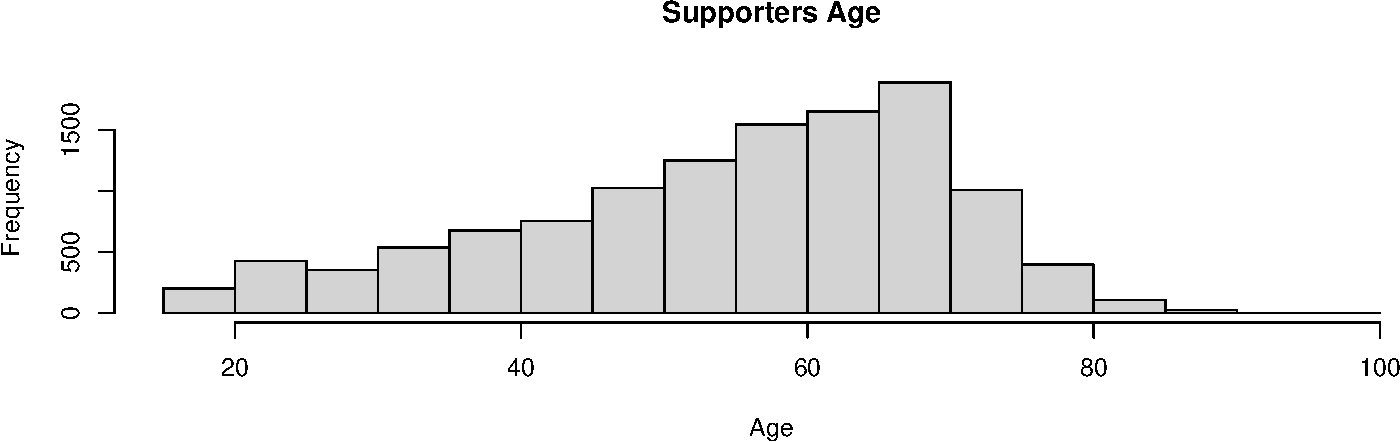
\includegraphics[height=0.4\textheight]{DSS_Ch03_files/figure-beamer/unnamed-chunk-8-1} \end{center}
\end{frame}

\begin{frame}[fragile]{記述統計量}
\protect\hypertarget{ux8a18ux8ff0ux7d71ux8a08ux91cf}{}
\begin{itemize}
\tightlist
\item
  分布の中心（平均値、中央値）とばらつき（標準偏差、分散）を計算する。
\end{itemize}

\begin{Shaded}
\begin{Highlighting}[]
\CommentTok{\# 離脱支持者の平均年齢}
\FunctionTok{mean}\NormalTok{(bes1}\SpecialCharTok{$}\NormalTok{age[bes1}\SpecialCharTok{$}\NormalTok{leave }\SpecialCharTok{==} \DecValTok{1}\NormalTok{])}
\end{Highlighting}
\end{Shaded}

\begin{verbatim}
## [1] 55.06823
\end{verbatim}

\begin{Shaded}
\begin{Highlighting}[]
\CommentTok{\# 離脱支持者の年齢の中央値}
\FunctionTok{median}\NormalTok{(bes1}\SpecialCharTok{$}\NormalTok{age[bes1}\SpecialCharTok{$}\NormalTok{leave }\SpecialCharTok{==} \DecValTok{1}\NormalTok{])}
\end{Highlighting}
\end{Shaded}

\begin{verbatim}
## [1] 58
\end{verbatim}

\begin{Shaded}
\begin{Highlighting}[]
\CommentTok{\# 標準偏差}
\FunctionTok{sd}\NormalTok{(bes1}\SpecialCharTok{$}\NormalTok{age[bes1}\SpecialCharTok{$}\NormalTok{leave }\SpecialCharTok{==} \DecValTok{1}\NormalTok{])}
\end{Highlighting}
\end{Shaded}

\begin{verbatim}
## [1] 14.96106
\end{verbatim}
\end{frame}

\hypertarget{ux6559ux80b2ux3068ux96e2ux8131ux6d3eux7968ux3068ux306eux95a2ux4fc2}{%
\section{3.5
教育と離脱派票との関係}\label{ux6559ux80b2ux3068ux96e2ux8131ux6d3eux7968ux3068ux306eux95a2ux4fc2}}

\begin{frame}[fragile]{散布図 (1)}
\protect\hypertarget{ux6563ux5e03ux56f3-1}{}
\begin{itemize}
\tightlist
\item
  地区レベルのデータを使用する。
\end{itemize}

\begin{Shaded}
\begin{Highlighting}[]
\CommentTok{\# 地区レベルデータの読み込み}
\NormalTok{dis }\OtherTok{\textless{}{-}} \FunctionTok{read.csv}\NormalTok{(}\StringTok{"UK\_districts.csv"}\NormalTok{)}
\NormalTok{dis1 }\OtherTok{\textless{}{-}} \FunctionTok{na.omit}\NormalTok{(dis)}
\end{Highlighting}
\end{Shaded}
\end{frame}

\begin{frame}[fragile]{散布図 (2)}
\protect\hypertarget{ux6563ux5e03ux56f3-2}{}
\begin{itemize}
\tightlist
\item
  \texttt{plot()} で2つの数値変数の関係をプロットする。
\item
  \texttt{abline()} で平均値を示す直線などを追加できる。
\end{itemize}

\footnotesize

\begin{Shaded}
\begin{Highlighting}[]
\FunctionTok{plot}\NormalTok{(dis1}\SpecialCharTok{$}\NormalTok{high\_education, dis1}\SpecialCharTok{$}\NormalTok{leave, }
     \AttributeTok{xlab =} \StringTok{"High Education (\%)"}\NormalTok{, }
     \AttributeTok{ylab =} \StringTok{"Leave Vote (\%)"}\NormalTok{)}
\FunctionTok{abline}\NormalTok{(}\AttributeTok{v =} \FunctionTok{mean}\NormalTok{(dis1}\SpecialCharTok{$}\NormalTok{high\_education), }\AttributeTok{lty =} \StringTok{"dashed"}\NormalTok{)}
\FunctionTok{abline}\NormalTok{(}\AttributeTok{h =} \FunctionTok{mean}\NormalTok{(dis1}\SpecialCharTok{$}\NormalTok{leave), }\AttributeTok{lty =} \StringTok{"dashed"}\NormalTok{)}
\end{Highlighting}
\end{Shaded}

\begin{center}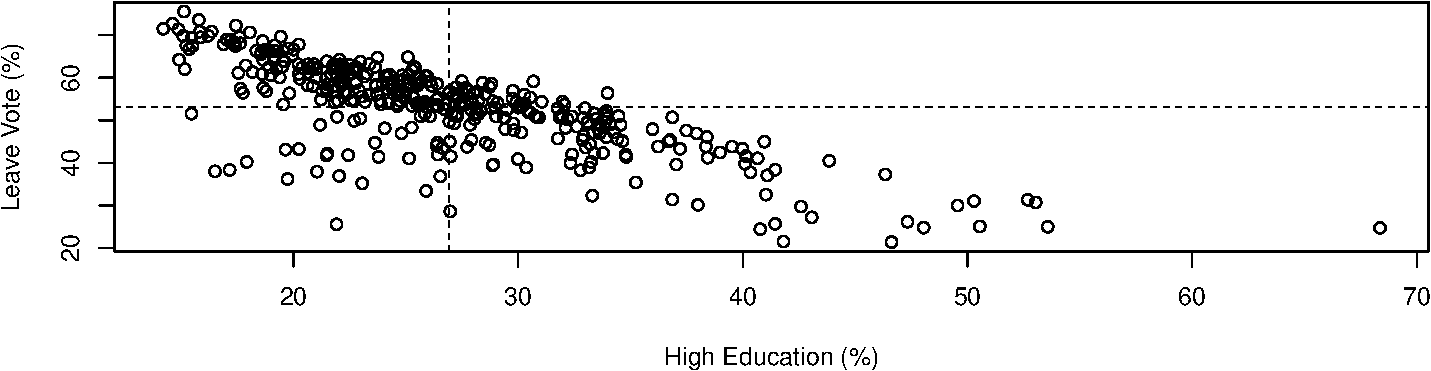
\includegraphics[height=0.4\textheight]{DSS_Ch03_files/figure-beamer/unnamed-chunk-11-1} \end{center}

\normalsize
\end{frame}

\begin{frame}[fragile]{相関}
\protect\hypertarget{ux76f8ux95a2}{}
\begin{itemize}
\tightlist
\item
  \texttt{cor()}
  で2つの変数の間の線形関係の強さと方向を数値化する（-1から1の間）。
\end{itemize}

\begin{Shaded}
\begin{Highlighting}[]
\CommentTok{\# 高学歴率と離脱派得票率の相関}
\FunctionTok{cor}\NormalTok{(dis1}\SpecialCharTok{$}\NormalTok{high\_education, dis1}\SpecialCharTok{$}\NormalTok{leave)}
\end{Highlighting}
\end{Shaded}

\begin{verbatim}
## [1] -0.7633185
\end{verbatim}

\begin{itemize}
\tightlist
\item
  \textbf{解釈}:
  強い負の相関がある。教育水準が高い地区ほど、離脱派の得票率が低い傾向にある。
\end{itemize}
\end{frame}

\hypertarget{ux307eux3068ux3081}{%
\section{3.6 まとめ}\label{ux307eux3068ux3081}}

\begin{frame}[fragile]{第3章のまとめ}
\protect\hypertarget{ux7b2c3ux7ae0ux306eux307eux3068ux3081}{}
\begin{itemize}
\tightlist
\item
  \textbf{測定}:
  母集団を代表する標本を用いて、関心のある数量を推定する。
\item
  \textbf{無作為抽出}: 推論の妥当性を高めるための基本的な手法。
\item
  \textbf{データの要約と視覚化}:

  \begin{itemize}
  \tightlist
  \item
    度数表、比率表、クロス表。
  \item
    ヒストグラム、散布図。
  \item
    平均、中央値、標準偏差、相関係数。
  \end{itemize}
\item
  \textbf{Rの操作}: \texttt{table()}, \texttt{prop.table()},
  \texttt{na.omit()}, \texttt{hist()}, \texttt{plot()}, \texttt{cor()}
  を学んだ。
\end{itemize}
\end{frame}

\end{document}
